% pdflatex presentation.tex & pdflatex presentation.tex

% created by Uwe Schadewald
% modified by Mathias Kuntze and Ahmet Uysal
% Add, handout to documentclass arguments for condensed pdf
\documentclass[presentation, 8pt, mathserif, t]{beamer} % , aspectratio=169
\usepackage[english]{babel}
\usepackage{pgf,graphicx}
\usepackage{amsmath, amssymb}
\usepackage[utf8]{inputenc}
\usepackage{lmodern}
\usepackage{palatino}
\usepackage{multimedia}
\usepackage{pgfpages} 
\usepackage{tikz}
\usepackage{datetime}
\pdfoptionpdfminorversion=5

\usepackage{caption}
\usepackage{subcaption}
% if else
\usepackage{ifthen}
% extend table options
\usepackage{tabularx} 
\usepackage{booktabs}
\usepackage{multicol}
\usepackage{multirow}
\usepackage{eso-pic}  % package to set background image
\usepackage[calc]{picture}

% Packages and stuff for ToDo list like itempoints
\usepackage{pifont}
\newcommand{\cmark}{\ding{51}}%
\newcommand{\xmark}{\ding{55}}%
\newcommand{\open}{$\square$}
\newcommand{\done}{\rlap{$\square$}{\raisebox{1pt}{\large\hspace{1.5pt}\cmark}}\hspace{-2.5pt}}
\newcommand{\wontfix}{\rlap{$\square$}{\raisebox{1pt}{\large\hspace{1.5pt}\xmark}}}
\newcommand{\notsure}{\rlap{$\square$}{\raisebox{0.8pt}{\large\hspace{1.5pt}\textbf{?}}}}



% side bar and footer
\setbeamertemplate{headline}{	
	\leavevmode
	\vspace{-4em}	
	\hbox{		
		\begin{beamercolorbox}[wd=0.85\paperwidth,ht=10ex,dp=8ex,center]{}%			
			% navigation with subsections as dots
			\hspace{3.5em}\insertnavigation{0.7\paperwidth}{\hskip0pt plus1fill} % add navigation in footer						
			% navigation with sections, no subsections
			% \insertsectionnavigationhorizontal{0.6\paperwidth}{\hskip0pt plus1fill}{} \\ % add navigation in footer}
			
		\end{beamercolorbox} 				
	}
	\vskip0pt
}


\setbeamertemplate{footline}{	
	\leavevmode
	\vspace{-3em}
	\hbox{
		\begin{beamercolorbox}[wd=.33\paperwidth,ht=2.25ex,dp=1ex,left]{author in head/foot}%
			\hspace{5em}
			\insertshortauthor
		\end{beamercolorbox}
		\begin{beamercolorbox}[wd=.33\paperwidth,ht=2.25ex,dp=1ex,center]{title in head/foot}%
			\insertshorttitle \ - \insertshortsubtitle
		\end{beamercolorbox}	
		\begin{beamercolorbox}[wd=0.30\paperwidth,ht=10ex,dp=8ex,right]{pagenumber in head/foot}			 	
			\insertframenumber % add page numbers
		\end{beamercolorbox}
	}			
	\vskip0pt
}



\setbeamertemplate{frametitle}{
	\ifthenelse{\equal{\insertframesubtitle}{}}{
		\vspace{0.6cm}
		\huge{\insertframetitle}
	}{
		\vspace{0.6cm}
		\small{\insertframetitle}\\
		\vspace{0.3cm}
		\huge{\insertframesubtitle}
    }		
}

	
% enumerate sections
\setbeamertemplate{section in head/foot}{\hfill\insertsectionheadnumber.~\insertsectionhead}
%\setbeamertemplate{section in head/foot shaded}{\color{structure!50}\hfill\insertsectionheadnumber.~\insertsectionhead}
\setbeamertemplate{section in toc}{\inserttocsectionnumber.~\inserttocsection}

%enumerate subsections
\setbeamertemplate{subsection in head/foot}{\hfill\insertsubsectionheadnumber.~\insertsubsectionhead}
\setbeamertemplate{subsection in head/foot shaded}{\color{structure!50}\hfill\insertsubsectionheadnumber.~\insertsubsectionhead}
%\setbeamertemplate{subsection in toc}[subsections numbered]
\setbeamertemplate{subsection in toc}{\vskip0.5em\leftskip=2em\inserttocsubsection\par}

%--------------------------Common------------------------------------------------------
\setbeamercovered{transparent} % make the beamer theme invisible
\usefonttheme{structurebold}
\beamertemplatenavigationsymbolsempty % set navigations helper function to off
\setbeamertemplate{bibliography item}[text]
\setbeamertemplate{note page}[plain]

%\setlist[itemize,1]{label={$\bullet$}} % \item are using bullets
\setbeamertemplate{itemize items}[circle]
	
	

	
% create a new command to show it on two screens
% I'm using dspdfviewer.
\newcommand{\setDualView} {
	\setbeameroption{show notes on second screen=right}
}

%\AtBeginSection[]{\subsection{}}
\newcommand{\addcite}[1]{%
	\AddToShipoutPictureFG*{%
		\AtPageLowerLeft{%
			\put(0.90\paperwidth,5em){											
				\tiny{
					\cite{#1} 
				}			
			}
		}
	}	
}

% insert a frame with references -> use bibtex
\newcommand{\insertReferenceFrame}[3]{%
	\section{#1}
	\begin{frame}[allowframebreaks]
		\frametitle{#1}
		\bibliographystyle{#2}
		\bibliography{#3}
	\end{frame}	
}

\AtBeginSection[]{\subsection{}}
	





\usepackage{../KU-Beamer-Template/style/koc} 

\title{KOLT Python} 
\subtitle{Program Information} 
\newdate{date}{21}{10}{2019}
\date{\displaydate{date}}
\author{Barış Tan}

\titlegraphic{\centering
\includegraphics[height=1.8cm]{images/vpaa_logo.png}
\includegraphics[height=1.4cm]{../KU-Beamer-Template/style/images/logo_kolt.pdf}}

\setbeamercovered{invisible} % transparent

\begin{document}
  \maketitle

	\frame{\frametitle{Agenda}\tableofcontents}

  \section{About}

    \begin{frame}
      \frametitle{About KOLT Python}
      
      \Large
      \begin{itemize}
        \item Founded in September 2018 with support of KOLT \& VPAA
        \item Accepted its first 20 students in Spring 2019
      \end{itemize}

      
    
    \end{frame}


    \begin{frame}
      \frametitle{Our Goals}
    
      
    
    \end{frame}


  \section{Team}
    \begin{frame}
      \frametitle{Team Members}
    
      \begin{columns}
				\column{5cm}
				\centering 
					
\includegraphics[width=2.25cm]{images/ahmet.jpg}\\
					Ahmet Uysal\\
					Senior Computer Eng.\\

          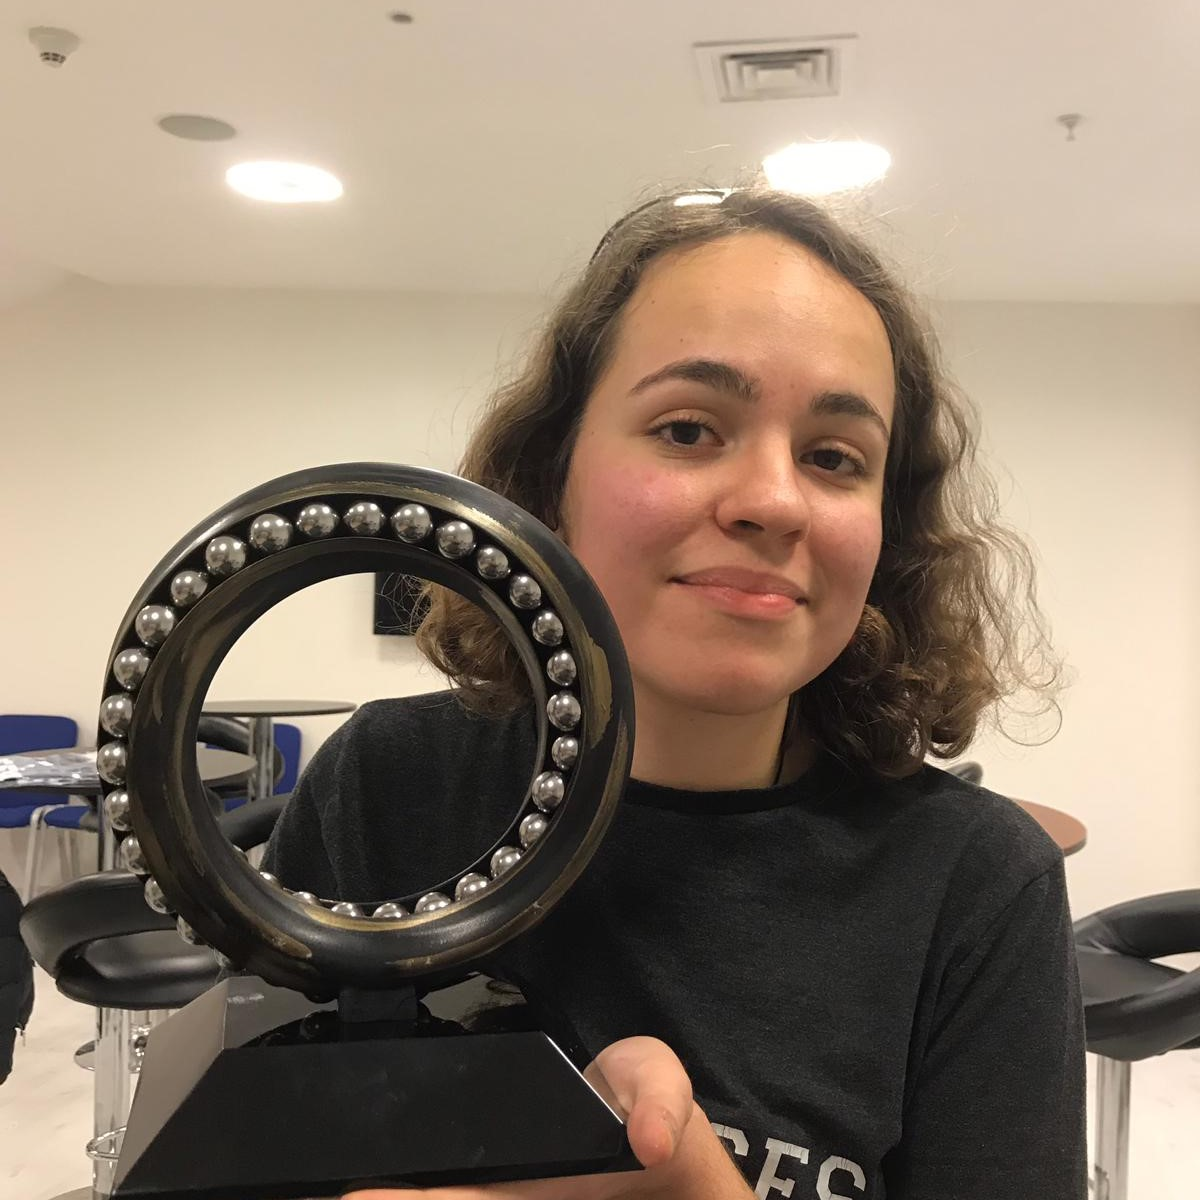
\includegraphics[width=2.25cm]{images/gulsena.jpg}\\
					Gül Sena Altıntaş\\
					Junior Comp. Eng. \& Math\\
				\column{5cm}
				\centering
					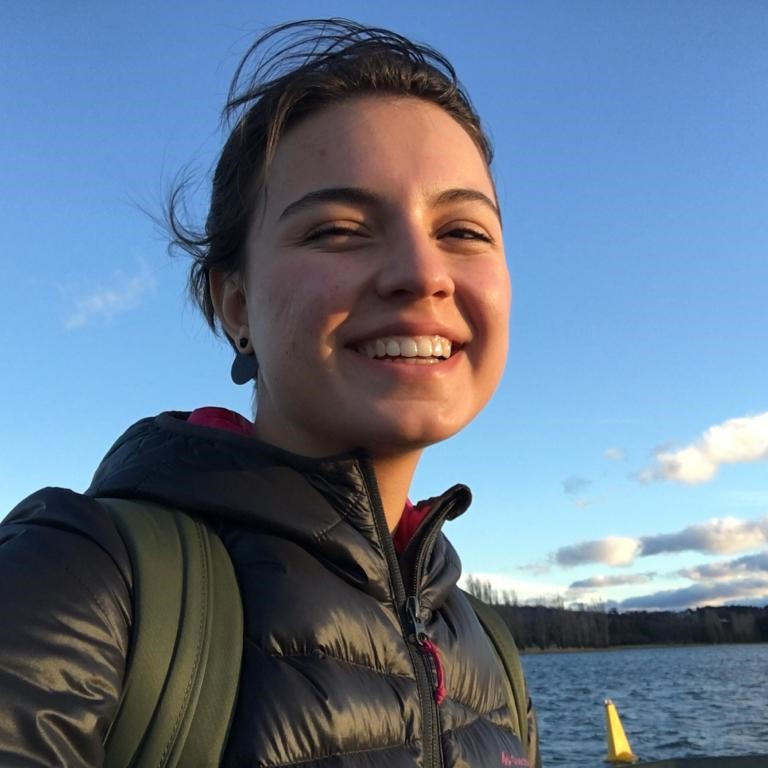
\includegraphics[width=2.25cm]{images/ceren.jpg}\\
					Ceren Kocaoğullar\\
					Senior Comp. Eng. \& MAVA
          
          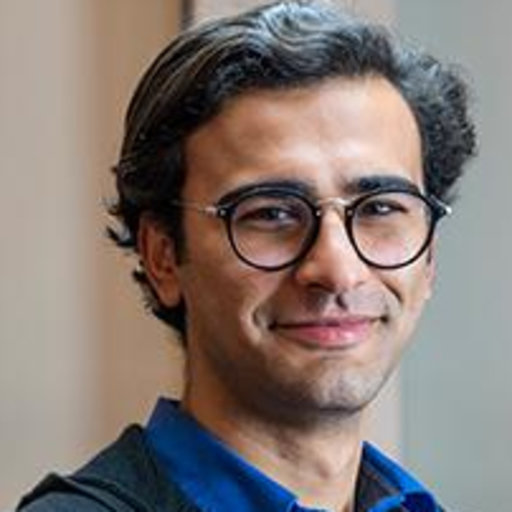
\includegraphics[width=2.25cm]{images/hasancan.jpg}\\
					Hasan Can Aslan\\
					Junior Comp. Eng. \& ECON
			\end{columns}
    
    \end{frame}


    \begin{frame}{Advisors}
    
      \begin{columns}
				\column{3.333cm}
				  \centering 
					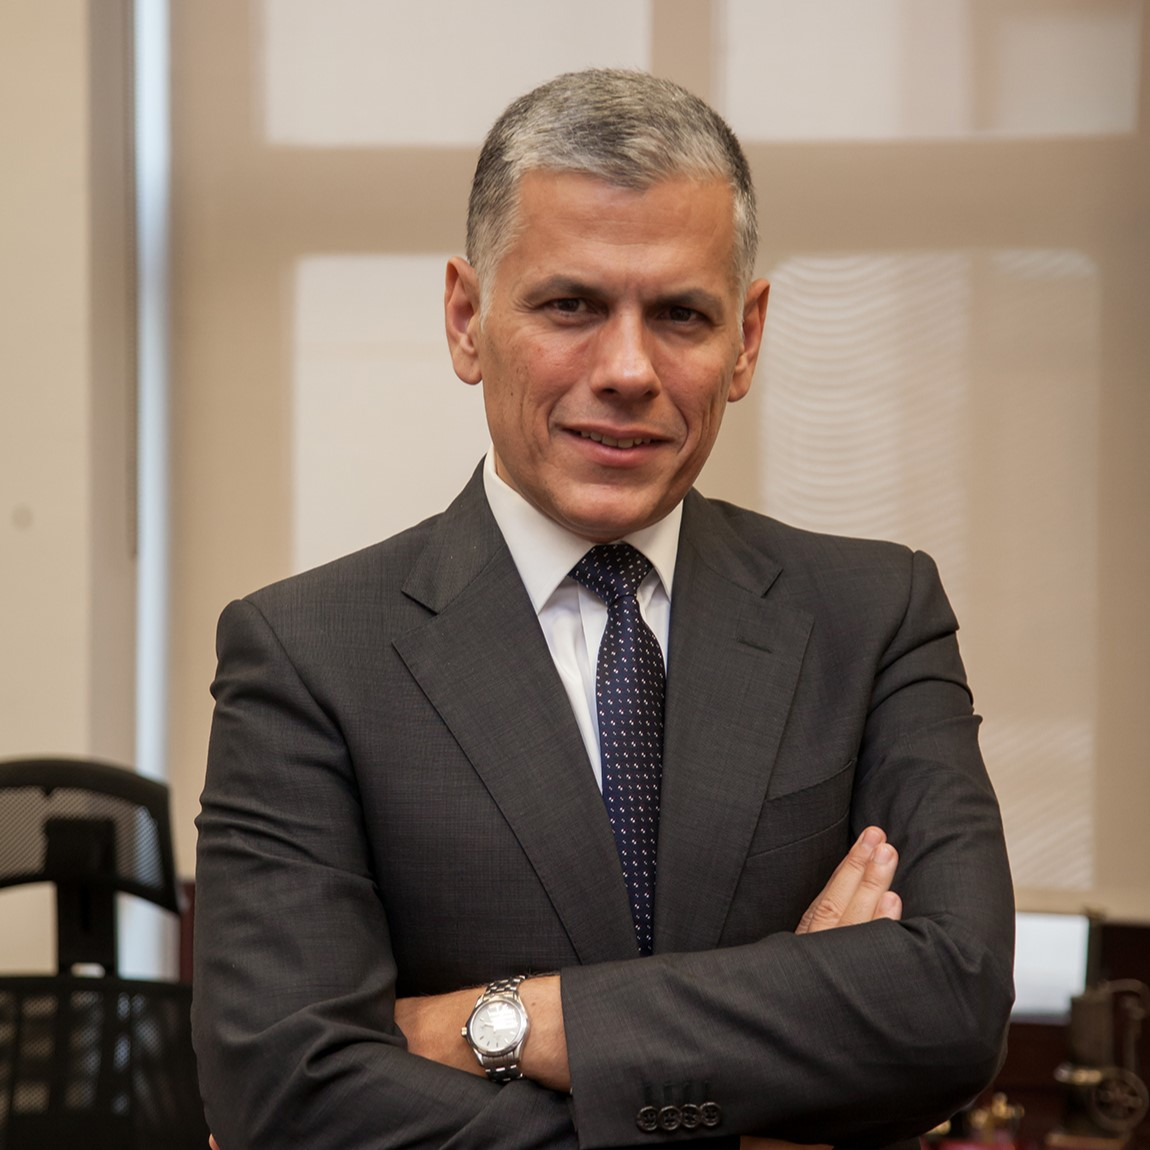
\includegraphics[width=2.5cm]{images/btan.jpg}\\
					Prof. Barış Tan\\
          \vspace{2.5mm}
          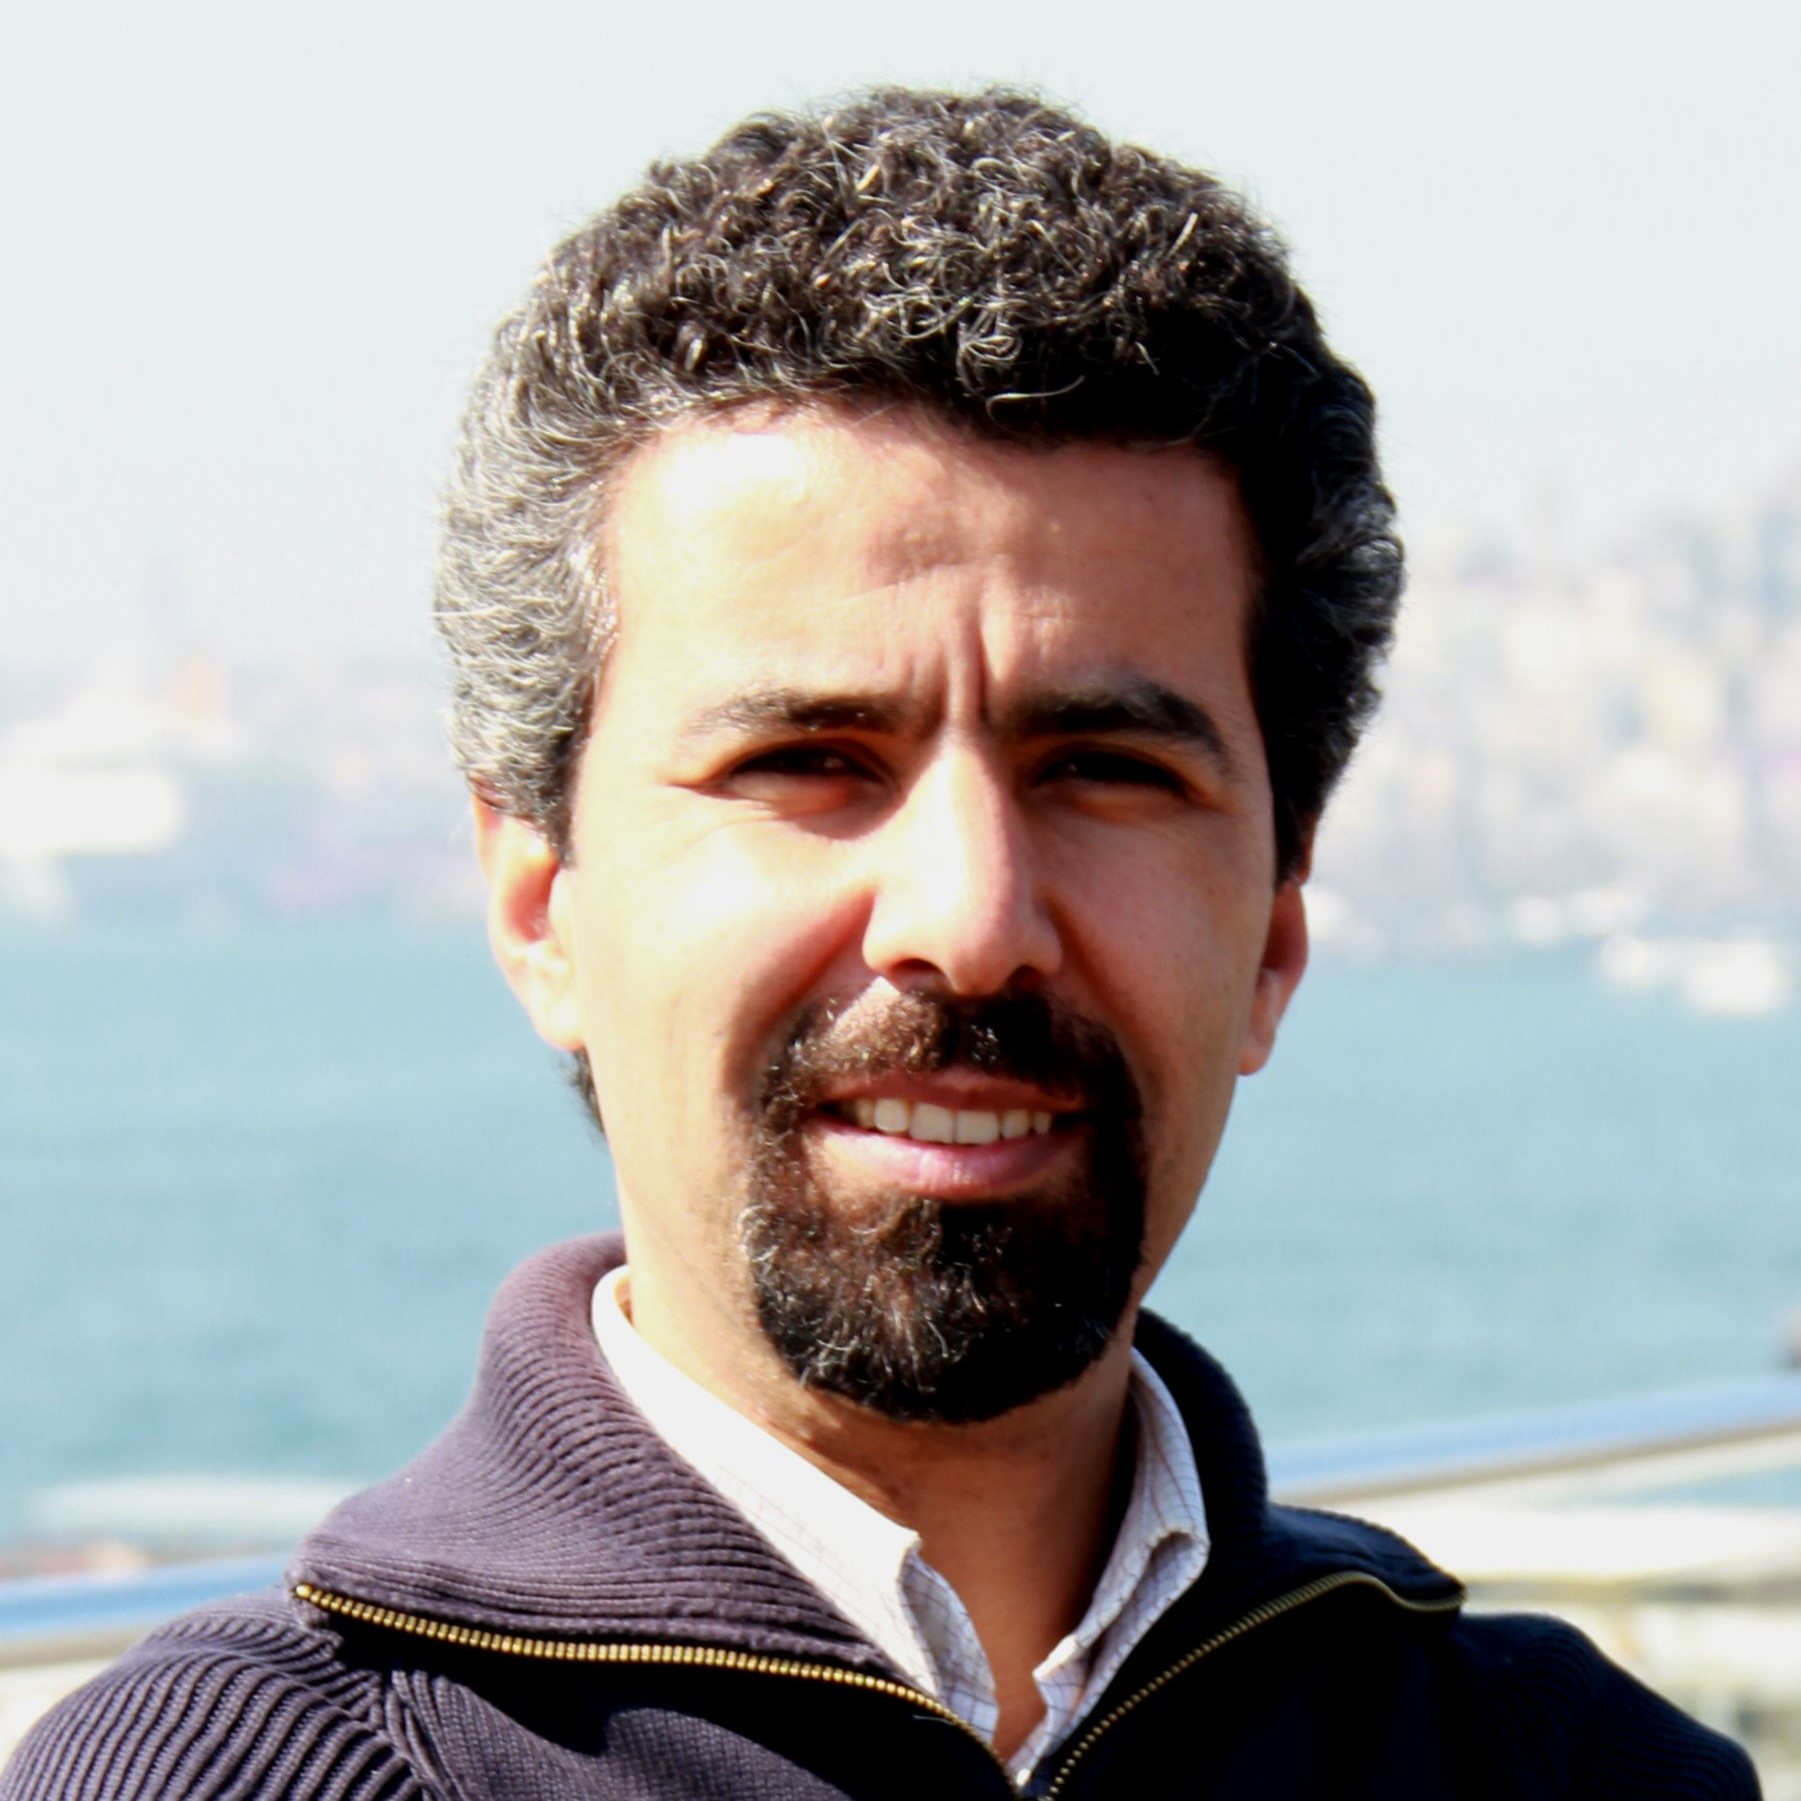
\includegraphics[width=2.5cm]{images/bbozkurt.jpg}\\
					Prof. Barış Bozkurt\\
        
          \column{3.333cm}
				  \centering
					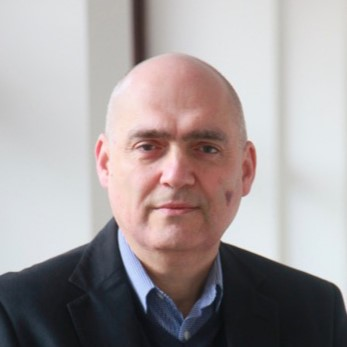
\includegraphics[width=2.5cm]{images/msozer.jpg}\\
					Prof. Murat Sözer\\
          \vspace{2.5mm}
          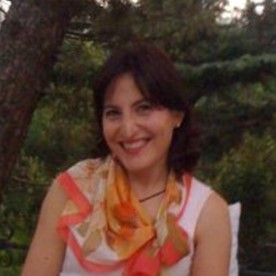
\includegraphics[width=2.5cm]{images/byobas.jpg}\\
					Dr. Banu Yobaş\\
          
        \column{3.333cm}
          \centering
          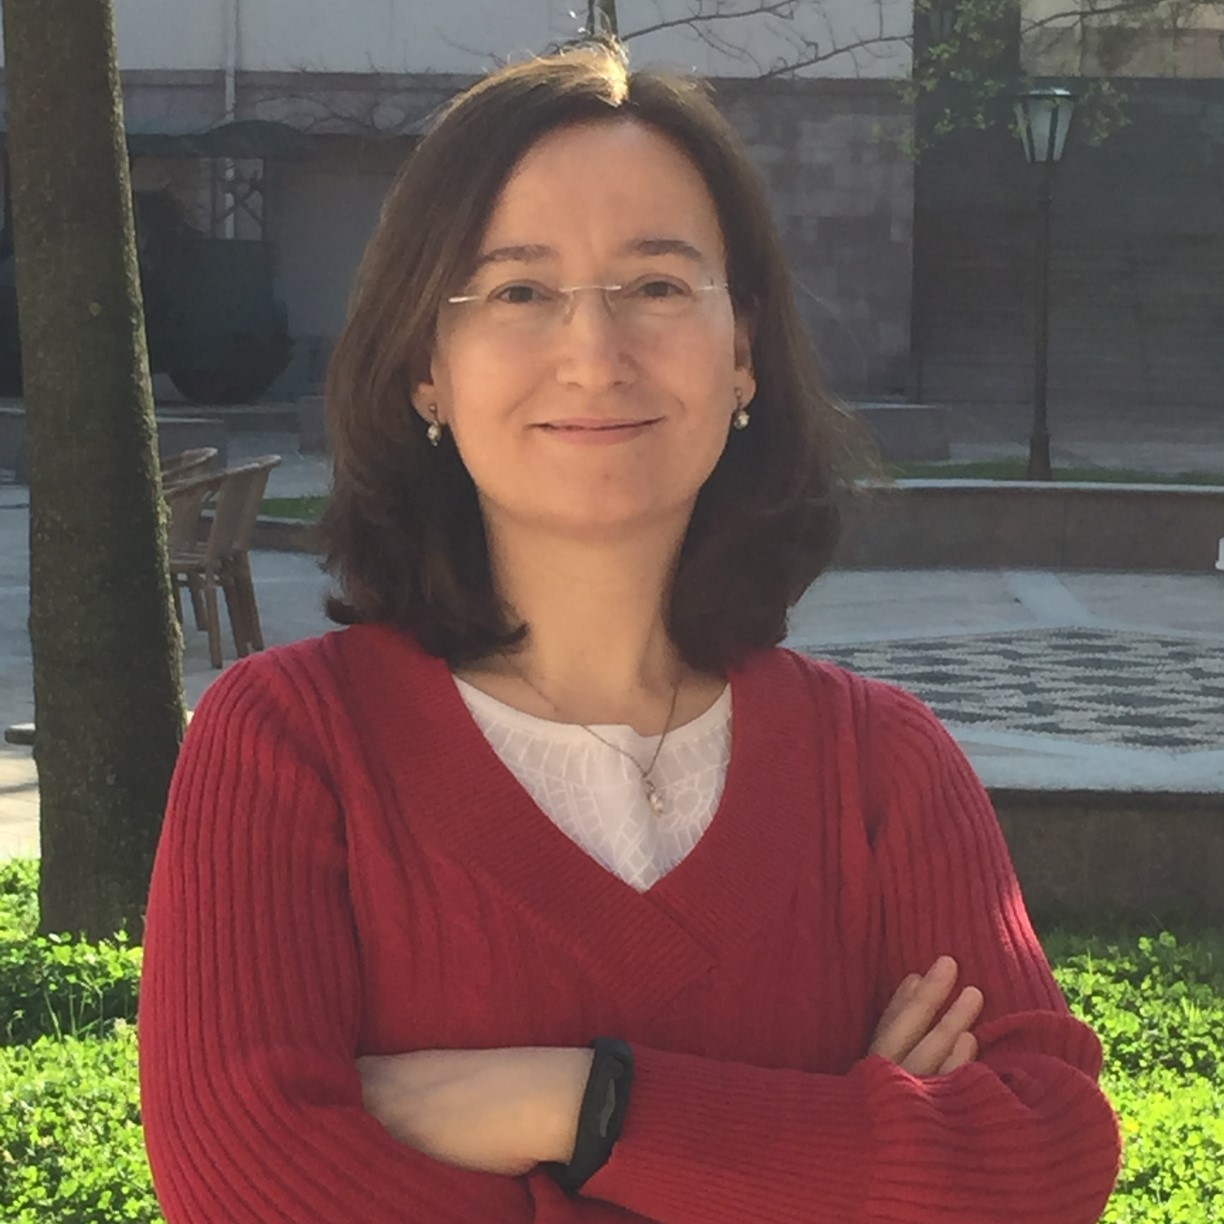
\includegraphics[width=2.5cm]{images/oozkasap.jpg}\\
          Prof. Öznur Özkasap\\
          \vspace{2.5mm}
          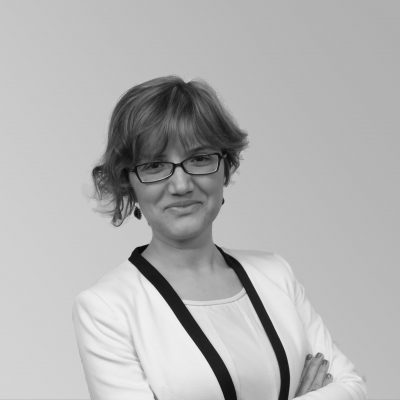
\includegraphics[width=2.5cm]{images/zzeybekoglu.jpg}\\
          Dr. Zuhal Zeybekoğlu\\
			\end{columns}
    
    \end{frame}

    \section{Certificate Program}

      \begin{frame}
        \frametitle{}
      
        
      
      \end{frame}



      \section{Student Reviews}

      \begin{frame}
        \frametitle{İrem Şot $\mid$ PhD $\mid$ Design, Technology \& Society}
        \vspace{-4mm}
        \begin{columns}
          \begin{column}{0.3\textwidth}
            \centering
            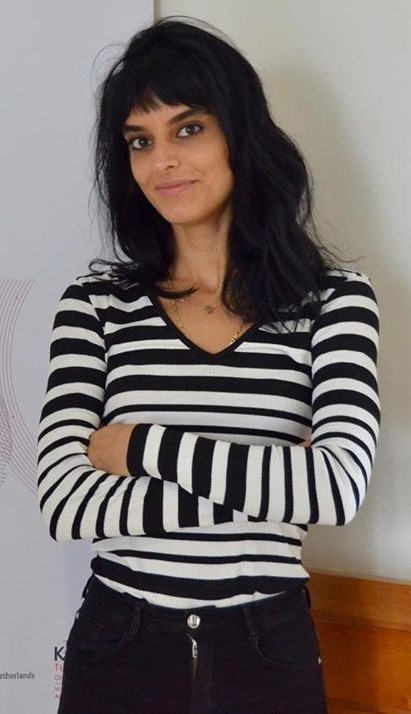
\includegraphics[width=\textwidth]{images/isot.jpg}
          \end{column}
          \begin{column}{0.7\textwidth}
            \begin{quote}
              As a person who caught up in Social Sciences for 10 years, I had several reservations before starting the KOLT Python Program. Apart from lacking any sort of knowledge about computer programming, the mere text-based education that I have obtained in the past years led me to question whether I would have been capable of learning the programming or not. Nevertheless, both the design of the program, and our trainers who allocate their spare time to our learning and employ rather simplistic and easy-to-grasp language made me realize that my thoughts regarding Python were just prejudice. Furthermore, the program is very lucrative in adopting participant oriented approach; lectures and sections are highly interactive, all material and exercise solutions are promptly made available online. This participant-centered approach surely facilitates asking the questions that most of us label as “embarrassing”.                          
            \end{quote}
          \end{column}
        \end{columns}
      \end{frame}

      \begin{frame}
        \frametitle{Mısra Taşçı $\mid$ Freshman $\mid$ School of Medicine}

        \begin{columns}
          \begin{column}{0.3\textwidth}
            \centering
            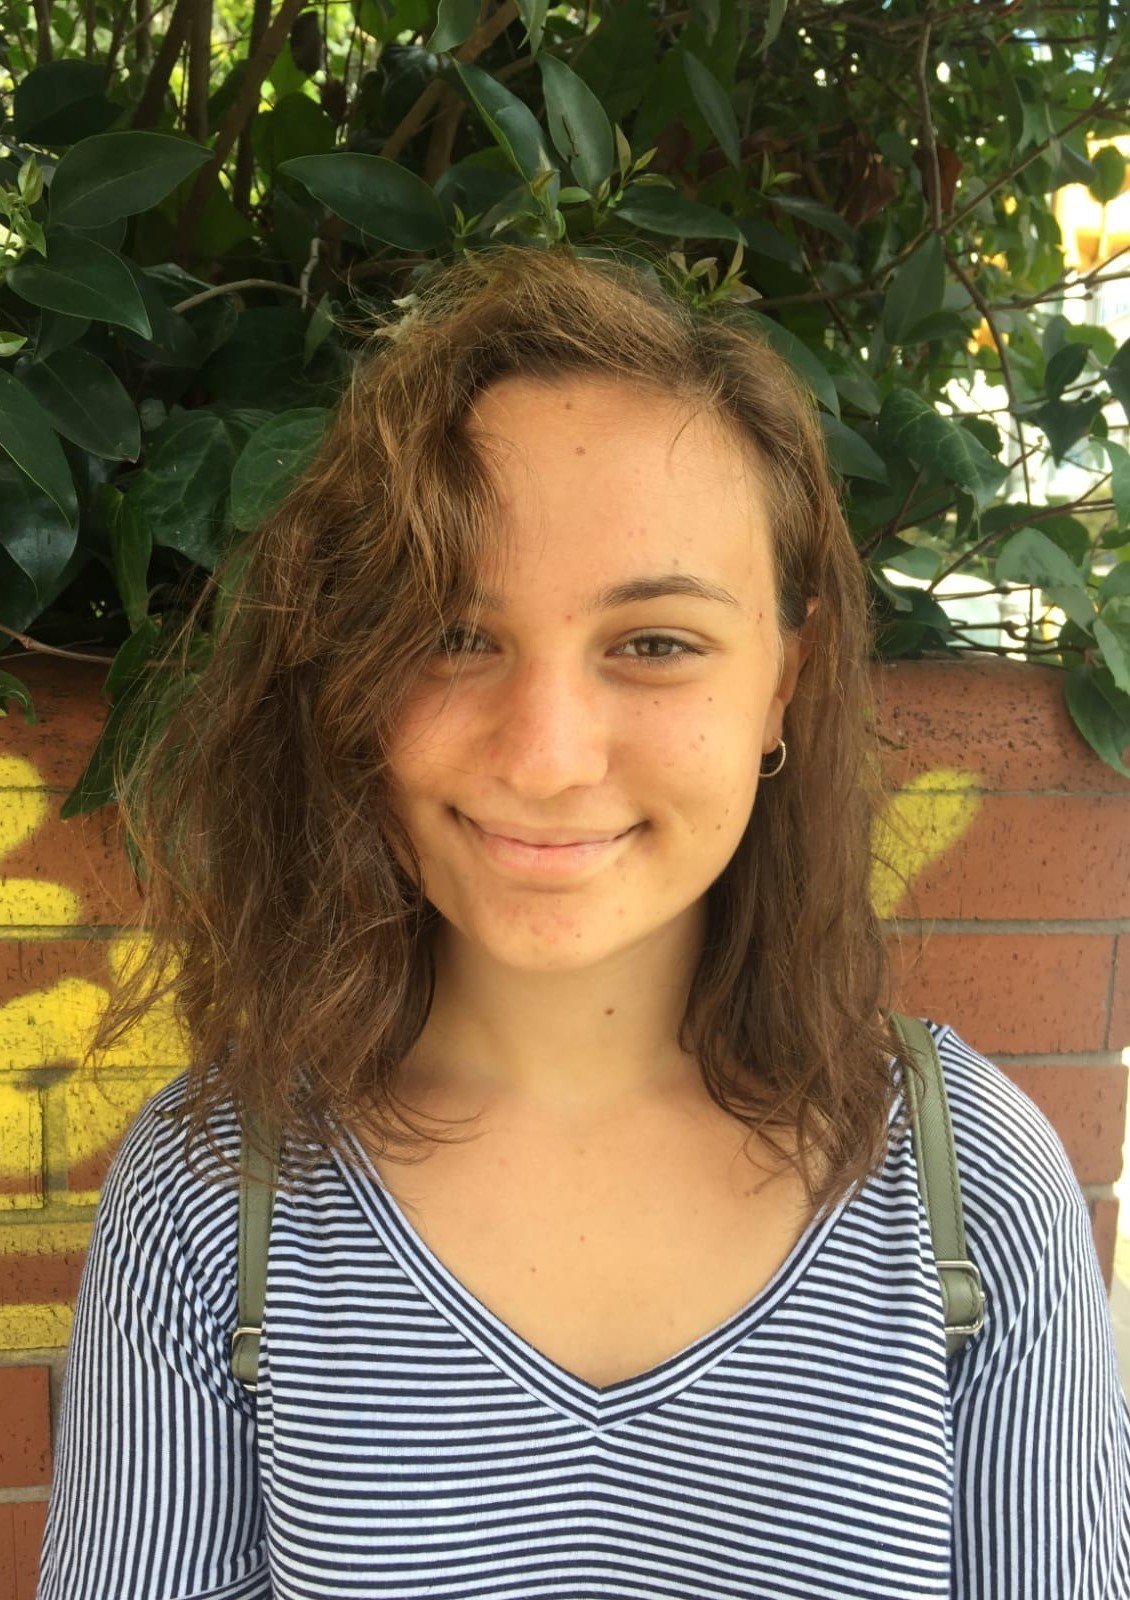
\includegraphics[width=\textwidth]{images/mtasci.jpg}
          \end{column}
          \begin{column}{0.7\textwidth}
            \Large
            \begin{quote}
            I'm a medical student and this is my first year. I am very interested in programming and this program is really great for me because it is like a serious course but it is fun and without the stress of exams. Also our instructors are very nice and helpful, and I really love the assignments that they prepare, time really passes quickly when I try doing them. I would love it if there were more programs like this about other subjects that I'm interested in.            \end{quote}
          \end{column}
        \end{columns}
      \end{frame}

      \begin{frame}
        \frametitle{Petrus J. Gerrits $\mid$ PhD $\mid$ Archeology}
        \begin{columns}
          \begin{column}{0.3\textwidth}
            \centering
            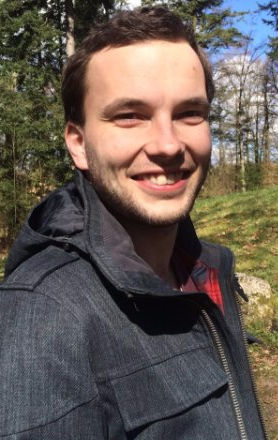
\includegraphics[width=\textwidth]{images/pgerrits.png}
          \end{column}
          \LARGE
          \begin{column}{0.7\textwidth}
            \begin{quote}
              The KOLT Python certificate program has been very useful for me so far. I studied Archaeology for my undergraduate and graduate studies and my hope is that with the content of this course I can make use of Python programming more regularly. The instructors are great, they make learning Python understandable, respond quickly to questions and assist whenever needed.
            \end{quote}
          \end{column}
        \end{columns}
      \end{frame}

\end{document}